% One-page explainer: Callaway and Sant'Anna (2021) and Sun and Abraham (2021).
% Build: cd 2_Documents && pdflatex cs_sa_one_pager.tex (run twice).
% Package facts checked on 21 October 2026 against did 2.5.1 and fixest 0.14.2.
\documentclass[10pt,letterpaper]{article}
\usepackage[T1]{fontenc}
\usepackage{mathptmx}
\renewcommand{\ttdefault}{lmtt} % Type 1 typewriter font (Latin Modern)
\usepackage[margin=0.75in]{geometry}
\usepackage{amsmath}
\usepackage[protrusion=false]{microtype} % keep all text inside the margins
\usepackage{multicol}
\usepackage{booktabs,tabularx,array}
\usepackage{ragged2e}
\usepackage{xcolor}
\usepackage{tikz}
\usetikzlibrary{arrows.meta}
\usepackage[font=normalsize,labelfont=bf,skip=2pt]{caption}
\usepackage{titlesec}
\usepackage[hidelinks]{hyperref}

\definecolor{okblue}{HTML}{0072B2} % Okabe-Ito blue
\titleformat{\section}{\normalsize\bfseries}{\thesection.}{0.4em}{}
\titlespacing*{\section}{0pt}{3pt}{1pt}
\setlength{\parindent}{0pt}
\setlength{\parskip}{1pt}
\setlength{\columnsep}{0.22in}
\setlength{\emergencystretch}{2em}
\pagestyle{empty}
\AtBeginDocument{%
  \setlength{\abovedisplayskip}{2pt}\setlength{\belowdisplayskip}{2pt}%
  \setlength{\abovedisplayshortskip}{1pt}\setlength{\belowdisplayshortskip}{1pt}}

\newcommand{\code}[1]{\texttt{#1}}
\newcommand{\ind}{\mathbf{1}}
\newcommand{\Cg}{\mathcal{C}}
\newcommand{\Gl}{\mathcal{G}_\ell}
\newcommand{\ATT}{\mathrm{ATT}}
\newcommand{\hATT}{\widehat{\mathrm{ATT}}}
\newcolumntype{P}[1]{>{\RaggedRight\arraybackslash}p{#1}}

\begin{document}

{\large\bfseries The Callaway and Sant'Anna (2021) and Sun and Abraham (2021) estimators\par}
\vspace{1pt}
For readers who know two-way fixed effects (TWFE) regression. CS: Callaway and Sant'Anna; SA: Sun and Abraham.

\begin{multicols}{2}
\section{The problem}
Unit $i$ starts treatment in period $G_i$ and stays treated ($G_i=\infty$ if never treated); cohort $g$ is the set of units with $G_i=g$, and $\ell=t-g$ is event time. The TWFE event-study regression is
\[
Y_{it}=\alpha_i+\lambda_t+\textstyle\sum_{\ell\neq-1}\mu_\ell\,\ind\{t-G_i=\ell\}+\varepsilon_{it}.
\]
With staggered adoption and effects that differ across cohorts, $\mu_\ell$ is a linear combination of cohort effects at event time $\ell$ and at other event times, so under parallel trends and no anticipation a lead ($\ell<0$) can differ from zero (SA). Goodman-Bacon (2021) shows that the static TWFE coefficient is a weighted average of all two-group, two-period difference-in-differences (DiD) estimates, including comparisons with an already-treated control cohort.

{\centering
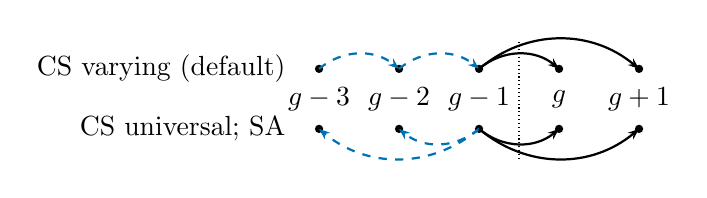
\begin{tikzpicture}[x=0.4in,y=0.3in,>={Stealth[length=4pt]}]
  \foreach \x/\lab in {0/{g-3},1/{g-2},2/{g-1},3/{g},4/{g+1}}
    \node at (\x,0.5) {$\lab$};
  \draw[densely dotted] (2.5,-0.5) -- (2.5,1.5);
  \node[anchor=east] at (-0.3,1) {CS varying (default)};
  \node[anchor=east] at (-0.3,0) {CS universal; SA};
  \foreach \y in {0,1} \foreach \x in {0,...,4} \fill (\x,\y) circle (1.5pt);
  \draw[->,okblue,dashed,thick] (0,1) to[bend left=40] (1,1);
  \draw[->,okblue,dashed,thick] (1,1) to[bend left=40] (2,1);
  \draw[->,thick] (2,1) to[bend left=40] (3,1);
  \draw[->,thick] (2,1) to[bend left=40] (4,1);
  \draw[->,okblue,dashed,thick] (2,0) to[bend left=40] (1,0);
  \draw[->,okblue,dashed,thick] (2,0) to[bend left=40] (0,0);
  \draw[->,thick] (2,0) to[bend right=40] (3,0);
  \draw[->,thick] (2,0) to[bend right=40] (4,0);
\end{tikzpicture}\par}
\captionof{figure}{Base periods for cohort $g$. An arrow from $b$ to $t$ marks the estimate for $t$ with base period $b$. Blue dashed: pre-treatment; black: post-treatment; dotted: treatment starts.}

\section{Callaway and Sant'Anna}
CS define $\ATT(g,t)=E[Y_t(g)-Y_t(0)\mid G=g]$, the average effect in period $t$ for cohort $g$, where $Y_t(g)$ and $Y_t(0)$ are potential outcomes under first treatment in $g$ and under no treatment. We estimate each one by a $2{\times}2$ DiD of mean outcomes $\bar Y$ between cohort $g$ and a comparison group $\Cg$, from a base period $b$ to $t$:
\[
\hATT(g,t)=(\bar Y_{g,t}-\bar Y_{g,b})-(\bar Y_{\Cg,t}-\bar Y_{\Cg,b}).
\]
$\Cg$ contains the never-treated units (did default) or the units not yet treated in $t$. For $t\ge g$, $b=g-1$. For $t<g$, $b=t-1$ with the varying base period (did default) and $b=g-1$ with the universal base period (Figure~1). With $K$ periods of anticipation, we use $g-1-K$ in place of $g-1$. Under parallel trends conditional on pre-treatment covariates, we estimate each comparison by outcome regression, inverse probability weighting, or doubly robust estimation; without covariates, the three coincide. For event time $\ell$, we average over the set $\Gl$ of cohorts observed at $\ell$, weighting by cohort size $n_g$:
\[
\hat\theta(\ell)=\textstyle\sum_{g\in\Gl}w_g(\ell)\,\hATT(g,g+\ell),\quad w_g(\ell)=n_g\big/\textstyle\sum_{h\in\Gl}n_h.
\]
In did, \code{att\_gt()} returns $\hATT(g,t)$ and \code{aggte()} returns $\hat\theta(\ell)$ with the dynamic aggregation (default: by cohort).

\section{Sun and Abraham}
SA estimate every $\mathrm{CATT}_{g,\ell}=\ATT(g,g+\ell)$ in one regression:
\[
Y_{it}=\alpha_i+\lambda_t+\textstyle\sum_{g\notin\Cg}\sum_{\ell\neq-1}\delta_{g,\ell}\,\ind\{G_i=g\}\,\ind\{t-G_i=\ell\}+\varepsilon_{it}.
\]
The control cohort $\Cg$ consists of the never-treated units or, if none exist, the last-treated cohort; SA then drop periods $t\ge\max_i G_i$. With reference period $\ell=-1$ for every cohort, $\hat\delta_{g,\ell}$ in a balanced panel equals the CS $2{\times}2$ DiD with universal base period $g-1$. The interaction-weighted estimator is $\hat\nu_\ell=\sum_{g\in\Gl}w_g(\ell)\,\hat\delta_{g,\ell}$. SA note that researchers can substitute covariate-adjusted CS estimates for $\hat\delta_{g,\ell}$. In fixest, \code{feols(y \raisebox{0.45ex}{\texttildelow} sunab(g, t) | id + t)} reports $\hat\nu_\ell$ by default.

\section{When the point estimates agree}
The CS and SA estimates of every $\ATT(g,t)$ and $\theta(\ell)$ are equal when the panel is balanced, there are no covariates, both comparison groups consist of the never-treated units, the CS base period is universal with zero anticipation, and the SA regression has an indicator for every event time except $-1$ (no binning; the fixest defaults). SA state that the two estimators coincide without covariates and with never-treated units.
\end{multicols}

\captionof{table}{CS versus SA in the papers, did 2.5.1 (\code{att\_gt()}, \code{aggte()}), and fixest 0.14.2 (\code{feols()} with \code{sunab()}). Point estimates depend on rows 1--5 (row 2: pre-treatment only) and agree when the choices match; rows 6--9 give package defaults for inference. $g$, $t$, $b$, $K$: cohort, period, base period, anticipation periods; IPW: inverse probability weighting.}
\vspace{-2pt}
\begin{tabularx}{\linewidth}{@{}P{1.4in}>{\RaggedRight\arraybackslash\hsize=1.12\hsize}X>{\RaggedRight\arraybackslash\hsize=0.88\hsize}X@{}}
\toprule
Setting & CS (did) & SA (paper; fixest)\\
\midrule
1. Comparison group & Never-treated (default) or not-yet-treated units & Never-treated, else last-treated cohort\\
2. Base period, $t<g$ & $b=t-1$ (varying, default) or $g-1$ (universal) & $b=g-1$\\
3. Covariates & Outcome regression, IPW, or doubly robust (default) & None; in fixest, covariates are regressors\\
4. No never-treated units & Last-treated cohort; periods before its treatment & Same (in fixest, we drop later periods)\\
5. Anticipation & $b=g-1-K$ for $K$ periods & We set reference event time $-1-K$\\
6. Standard errors & Multiplier bootstrap, 1,000 draws & Analytic; homoskedastic errors\\
7. Clustering & By unit & None (the default since version 0.13.0)\\
8. 95\% intervals & Simultaneous band over all reported estimates & Pointwise\\
9. Variation in weights & Included in event-study standard errors & Not included (fixed sample shares)\\
\bottomrule
\end{tabularx}

\vspace{3pt}
\textbf{References.} Berg\'e, L. (2026). fixest: Fast Fixed-Effects Estimations. R package version 0.14.2, CRAN. \enspace\textbullet\enspace
Callaway, B., and P. H. C. Sant'Anna (2021). Difference-in-Differences with multiple time periods. \emph{Journal of Econometrics} 225(2), 200--230. doi:10.1016/j.jeconom.2020.12.001. \enspace\textbullet\enspace
Callaway, B., and P. H. C. Sant'Anna (2026). did: Difference in Differences. R package version 2.5.1, CRAN. \enspace\textbullet\enspace
Goodman-Bacon, A. (2021). Difference-in-differences with variation in treatment timing. \emph{Journal of Econometrics} 225(2), 254--277. doi:10.1016/j.jeconom.2021.03.014. \enspace\textbullet\enspace
Sun, L., and S. Abraham (2021). Estimating dynamic treatment effects in event studies with heterogeneous treatment effects. \emph{Journal of Econometrics} 225(2), 175--199. doi:10.1016/j.jeconom.2020.09.006.

\end{document}
